\chapter{Prescripción de \emph{Feynman}}
\label{T38}
	
\begin{tikzpicture}
	\fill [left color=red!50, right color=teal!50] (0,0) rectangle (6.5,.1);
	\fill [left color=teal!50, right color=blue!50] (6.5,0) rectangle (11.5,.1);
	\end{tikzpicture}

\vspace{10mm}
\begin{adjustwidth}{50pt}{50pt}
\begin{ejemplo}
\vspace{2mm}

En este capítulo nos dedicaremos al cálculo de la siguiente ntegral:

$$\boldsymbol { \displaystyle \int_{-\infty}^{+\infty} \dfrac{e^{-iax}}{x^2-b^2}  \, \dd x} \quad a\in \mathbb R\, , \ b>0$$

Esta integral no existe, diverge, porque en el denominador hay dos puntos, $\pm b$, que lo anulan. Aparece que el cálculo de la función de Green de Feynman, que será el propagador de la QFT, por lo que debemos intentar resolverla.

Cuando una integral no converge, siempre podemos inventarnos el \underline{valor} \underline{principal} de Cauchy que consiste en deformar ligeramente el contorno con unas circunferencias de radio $\varepsilon$ rodeando a los ceros del denominador y, luego, hacer tender $\varepsilon$ a $0$. Si existe ese límite se obtiene un valor de la integral que tiene consistencia y sentido.
Luego está la \underline{prescripción} \underline{de} \underline{Feynman} que es una técnica de regularización y será la que adoptemos.\footnote{Se recomienda ver los capítulos 16 (integral de contorno) y 17 (parte principal de una integral) del curso `Teoría cuántica de Campos', de \emph{Javier García}.}
\vspace{2mm}
\end{ejemplo}
\end{adjustwidth}

\vspace{5mm}

\section{Parte principal}

\textcolor{gris}{Serie muy conveniente recordar algo de integración en $\mathbb C$.}

En análisis complejo, un \textbf{polo} de una función compleja de variable compleja es un cierto tipo de singularidad que se comporta como la singularidad $\ \dfrac 1 {z^n} \ $ en $z = 0\, .  \ $ 
\underline{Ejemplo}: La función $f(z)=\dfrac{z^2+1}{(z-2)(z+3)^4}$ tiene en $z_1=2$ un \emph{polo de orden 1} y en $z_2=-3$ un \emph{polo de orden 4}.


Se llama \textbf{Residuo} de $f(z)$  en $z_0$, un polo de orden $n$, a la expresión:

$$\boldsymbol{ Res(\, f(z)\, , \, z_0\, ) \ = \ \lim_{z\to z_0}\ \dfrac 1{(n-1)!}\ \dv[n-1]{z} \ \left( \, (z \to z_0)^n \cdot f(z) \, \right) } $$

Extendiendo la función de nuestra integral a todo el plano complejo, $\ f(z)=\dfrac{e^{-iaz}}{z^2-b^2} \, , \ $ y buscando los polos, vemos que $z_1=b$ y $z_2=-b$ son los dos polos de orden 1 de esta función, que podemos escribir como $ \ f(z)=\dfrac{e^{-iaz}}{(z-b)(z+b)}\, .$

Calculemos los resíduos: $\quad \displaystyle \Res(f(z),z_1)=\lim_{z \to z_0} \dfrac 1{(1-1)!}\, \dv[0]{z} (\, (z-z_1)^1\, f(z) \, ) \, = \, (z-z_1)\, f(z)\, ; \ $ para $z_2\, , \ \ \Res(f(z),z_1) =  (z-z_2)\, f(z) \, , \ $ al ser los dos polos de orden uno \textcolor{gris}{(la derivada de orden cero es como no derivar y 0!=1)}
 

$\boldsymbol{ \Res(f(z),b)=}\lim_{z\to b} \cancel{(z-b)} \dfrac{e^{-iaz}}{\cancel{(z-b)}(z+b)}=\boldsymbol{\dfrac{e^{-iab}}{2b}}\, ; \qquad \qquad \boldsymbol{\Res(f(z),-b)=-\dfrac{e^{iab}}{2b}}$


\vspace{5mm}\textbf{Teorema de residuos}

\begin{multicols}{2}

$$\displaystyle \oint_\gamma \, f(z)\, \dd z \ = \ 2\pi\, i\, \sum \text{ residuos interiores}$$

Si el giro es en el sentido horario, aparece un signo menos.
 \begin{figure}[H]
	\centering
	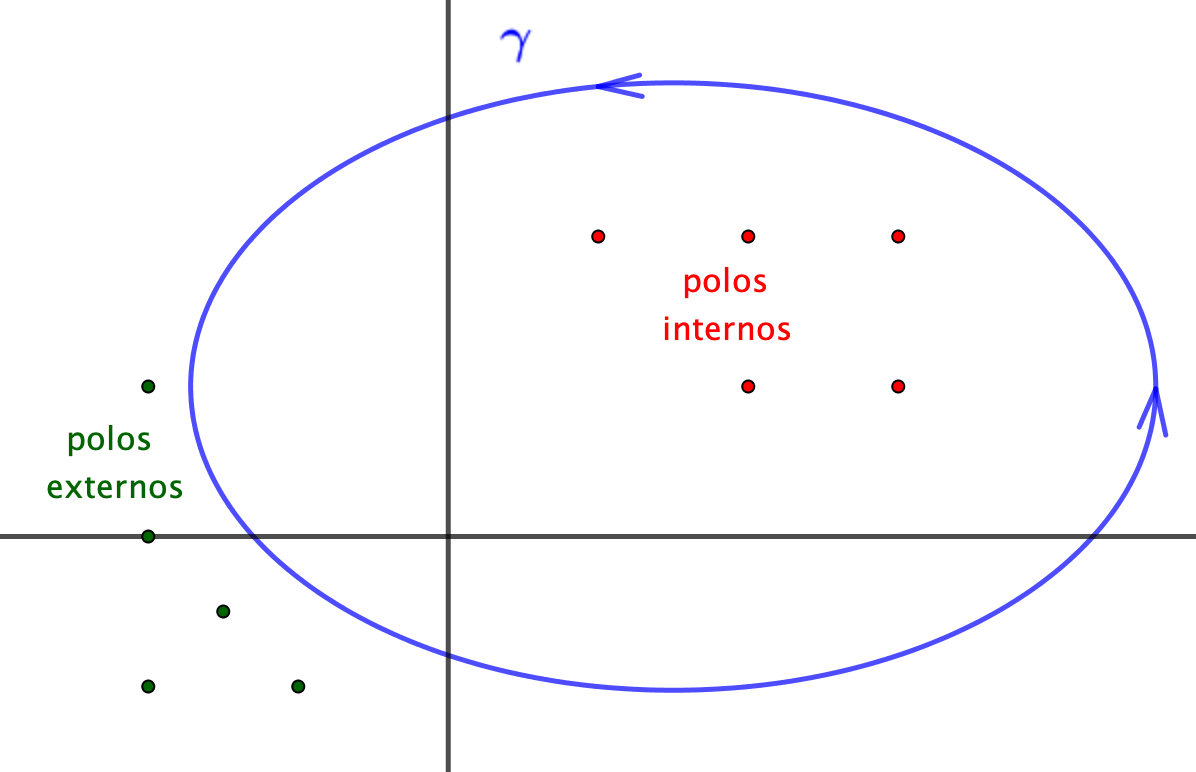
\includegraphics[width=.35\textwidth]{imagenes/img43-01.png}
\end{figure}	
\end{multicols}


\begin{multicols}{2}
 \begin{figure}[H]
	\centering
	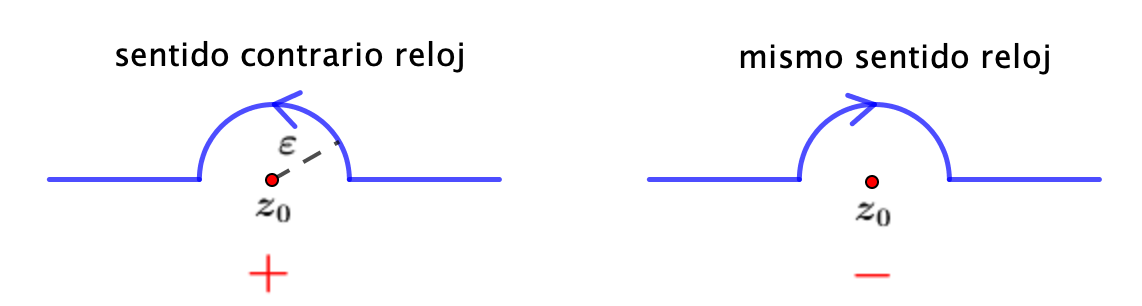
\includegraphics[width=.5\textwidth]{imagenes/img43-02.png}
\end{figure}

Contorno semicircular para el cálculo de una integral real: se rodea el polo con un semicírculo de radio $\varepsilon$ y luego se toma el límite cuando $\varepsilon \to 0$

En este caso:	
\end{multicols}
$\displaystyle \int\, f(z)\, \dd z \ = \ \pi\, i\, Res(\, f(z),z_0\, )\, . \quad$
Si el giro es en el sentido horario, aparece un signo menos.


\vspace{5mm} \textbf{Parte principal}

Es un medio de asociar un número, de algún modo, a la integral que queremos calcular y que sabemos que no existe:

$$\boldsymbol { \displaystyle \int_{-\infty}^{+\infty} \dfrac{e^{-iax}}{x^2-b^2}  \, \dd x} \quad a\in \mathbb R\, , \ b>0$$

\vspace{5mm}

\underline{Caso A}: 

Calculamos $\ \displaystyle \oint_\gamma \dfrac{e^{-1az}}{z^2-b^2}\ $ con un circuito $\gamma$ que rodee los polos del eje real por arriba con semicírculos de radio $\varepsilon \to 0$ y completamos por arriba del eje $x$ con un semicírculo de radio $R\to \infty$

$\displaystyle \oint_\gamma \dfrac{e^{-1az}}{z^2-b^2} = 2\pi\, i \, \sum \{ \text{ Residuos internos } \} =0$

Descomponemos la integral en 4 partes: 

\begin{multicols}{2}
 \begin{figure}[H]
	\centering
	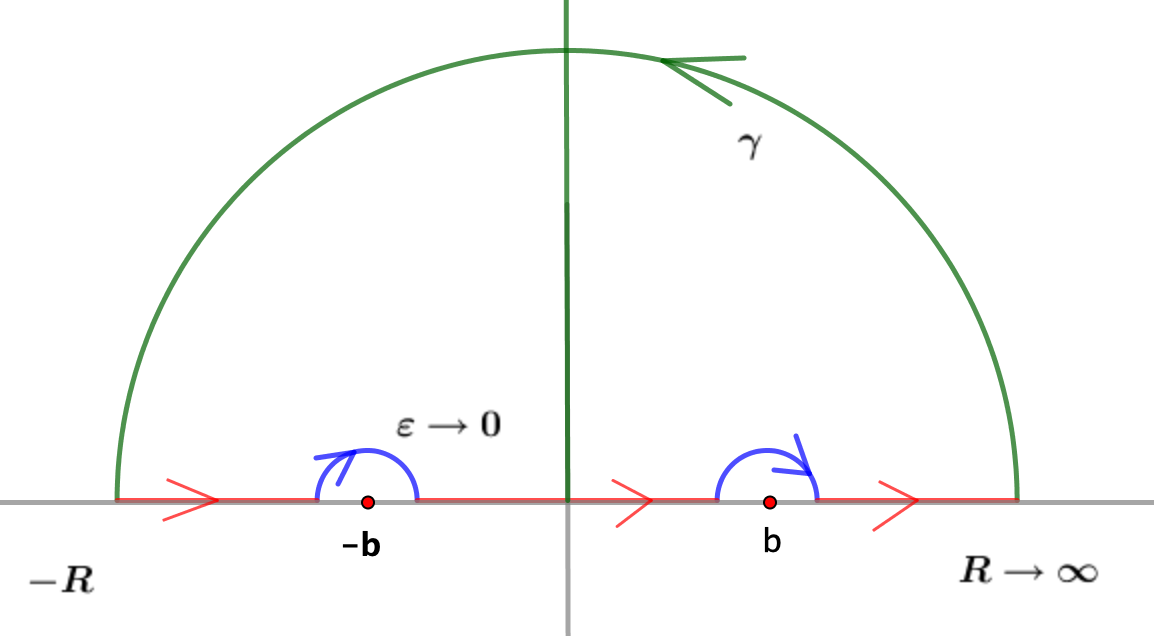
\includegraphics[width=.5\textwidth]{imagenes/img43-03.png}
\end{figure}
Descomponemos la integral en 4 partes: 

$\boldsymbol{ \quad I(\gamma) \ = \ \textcolor{red}{I(\mathbb R)} \ + \ \textcolor{blue}{I(-b;\, \varepsilon\to 0)} \ + }$

$\boldsymbol{ \qquad \qquad  + \ \textcolor{blue}{I(b;\, \varepsilon\to 0)} \ + \ \textcolor{green}{I(R\to \infty)} }$

\textcolor{red}{$I$} es la \textbf{parte principal} o \emph{valor principal de Cauchy}
\end{multicols}


$0=I-\pi i \Res(f(z),-b) -\pi i \Res(f(z),b) + 0^* \qquad \qquad 0 = I -\pi i \left( \dfrac{e^{iab}}{-2b} \right) -\pi i \left( \dfrac{e^{-iab}}{2b}  \right) + 0^*$

$ *  \quad R \to \infty \quad  R>0:\ \theta\in [0,\pi],\ \boldsymbol{a<0} \ \ $ entonces $e^{-iaz}\to 0\ $ y $\ $ \textcolor{green}{$I$}$=0$.

\textcolor{gris}{$*\quad  e^{-iaz}=e^{-iaR(cos\theta + i \sin \theta}=e^{-iaR\cos \theta)} \, e^{aR \sin \theta} \qquad R\to \infty \, \wedge \, a<0 \Rightarrow  e^{aR \sin \theta} \to 0 \, \Rightarrow \, \textcolor{green}{I}=0$}



Despejando, $\displaystyle \quad  I  = \dfrac{\pi i}{2b}\, (\, e^{-iab}-e^{iab} \,) = \dfrac{\pi i}{2b}\, [(\cos(ab)-i\sin(ab))-(\cos(ab)+i\sin(ab))] = \dfrac{\pi i}{2b}\, (-2i \sin(ab))$

$\boldsymbol{I\ = \ \dfrac \pi b \, \sin (ab)} \qquad \qquad a<0,\ \  b>0$




A $\boldsymbol I$ se le llama \textbf{parte principal} o \emph{valor principal de Cauchy} de la integral $\ \displaystyle PV\, \int_{-\infty}^{+\infty} \dfrac{e^{-iax}}{x^2-b^2}  \, \dd x$



Hemos obtenido que si rodeamos los polos de orden uno por arriba con semicircunferencias de radio $\varepsilon\to 0$ y cerramos el circuito por arriba con una semicircunferencia de radio $R\to \infty$, al imponer que $\boldsymbol{a<0}$ obtenemos que $\ \displaystyle \boldsymbol{ PV\, \int_{-\infty}^{+\infty} \dfrac{e^{-iax}}{x^2-b^2}  \, \dd x =  \dfrac \pi b \, \sin (ab) }$


\vspace{5mm}
	
\underline{Caso B}: 

Calculamos $\ \displaystyle \oint_\gamma \dfrac{e^{-1az}}{z^2-b^2}\ $ con un circuito $\gamma$ que rodee los polos del eje real por abajo con semicírculos de radio $\varepsilon \to 0$ y completamos por abajo del eje $x$ con un semicírculo de radio $R\to \infty$


$\displaystyle \oint_\gamma \Rightarrow 2\pi\, i \, \sum \{ \text{ Residuos internos } \} = 2\pi \, i \, \left( \, Res(-b,f(z))º + \ Res(b,f(z) \, \right) = 2\pi \, i \ \left[\,  \dfrac{e^{-iab}}{2b}\, - \,  \dfrac{e^{iab}}{2b} \, \right]$

$=\displaystyle -\dfrac{2\pi\, i}{2b} \, \left( \dfrac{e^{iab}-e^{-iab}}{2i}\, (2i) \right) = \dfrac {2\pi}b \, \sin(ab)$


\newpage %********************************

\hspace{2cm} %******************************

Descomponemos la integral en 4 partes: 

\begin{multicols}{2}
 \begin{figure}[H]
	\centering
	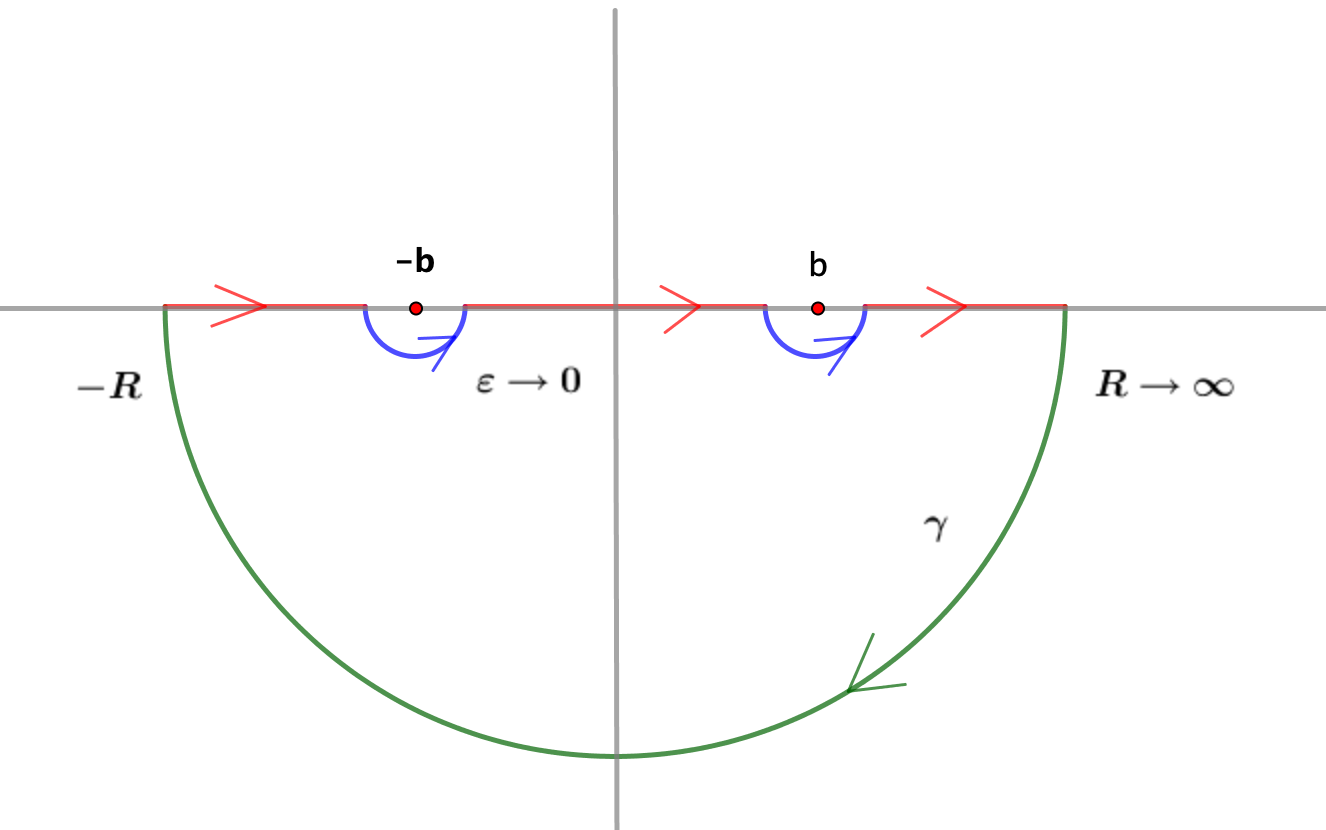
\includegraphics[width=.5\textwidth]{imagenes/img43-03bis.png}
\end{figure}
Descomponemos la integral en 4 partes: 

$\boldsymbol{ \quad I(\gamma) \ = \ \textcolor{red}{I(\mathbb R)} \ + \ \textcolor{blue}{I(-b;\, \varepsilon\to 0)} \ + }$

$\boldsymbol{ \qquad \qquad  + \ \textcolor{blue}{I(b;\, \varepsilon\to 0)} \ + \ \textcolor{green}{I(R\to \infty)} }$

$\dfrac{2\pi}b \sin(ab) = I -\pi i \left( \dfrac{e^{iab}}{-2b} \right) -\pi i \left( \dfrac{e^{-iab}}{2b}  \right) + 0$

$*  \quad R\to \infty \quad  \boldsymbol{a>0} \ \ $ para que $e^{-iaz}\to 0$

\end{multicols}

$ *  \quad R \to \infty \quad  R>0:\ \theta\in [\pi,2\pi],\ \sin\theta<0,\ \boldsymbol{a>0} \ \ $ entonces $e^{-iaz}\to 0\ $ y $\ $ \textcolor{green}{$I$}$=0$.


\begin{small} \textcolor{gris}{$*\quad  e^{-iaz}=e^{-iaR(cos\theta + i \sin \theta)}=e^{-iaR\cos \theta} \, e^{aR \sin \theta} \qquad R\to \infty \, \wedge \, a>0 \, \wedge \sin\theta<0 \Rightarrow  e^{aR \sin \theta} \to 0 \, \Rightarrow \, \textcolor{green}{I}=0$} \end{small}

$\dfrac{2\pi}{b} \sin (ab) \ = \  I \ - \  \dfrac{\pi i }{2b} \left( \dfrac{e^{iab}}{-2b} \right) \ - \    \dfrac{\pi i }{2b} \left( \dfrac{e^{-iab}}{-2b} \right) \ + \  0 \qquad \qquad \boldsymbol{a>0}$


$I=\dfrac{2\pi}{b} \sin (ab) - \dfrac{\pi i}{2b} e^{iab} + \dfrac{\pi i}{2b} e^{-iab} = \dfrac{2\pi}{b} \sin (ab) - \dfrac{\pi i}{2b} \left( e^{iab} - e^{-iab}  \right) = $

$ = \dfrac{2\pi}{b} \sin (ab) - \dfrac{\pi i}{2b} \left( \dfrac{e^{iab} - e^{-iab}}{2i}  \right)\, (2i)= \dfrac{2\pi}{b} \sin (ab) - \dfrac{\pi}{b} \sin (ab) = \dfrac{\pi}{b} \sin (ab)$

\vspace{15mm} %****************************************
$\boldsymbol I$ es la  \textbf{parte principal} o \emph{valor principal de Cauchy} de la integral $\ I=PV\,  \displaystyle \int_{-\infty}^{+\infty} \dfrac{e^{-iax}}{x^2-b^2}   $

Hemos obtenido que si rodeamos los polos de orden uno por abajo con circunferencias de radio $\varepsilon \to 0 $ y cerramos el circuito por abajo con una semicircunferencia de radio $R\to \infty$, al imponer que $\boldsymbol{a>0}$ obtenemos que $\ \displaystyle \boldsymbol{ PV\, \int_{-\infty}^{+\infty} \dfrac{e^{-iax}}{x^2-b^2}  \, \dd x =  \dfrac \pi b \, \sin (ab) } $


\vspace{15mm} %****************************************
?`Cómo es que ahora no da cero, da el mismo resultado? Incluso aunque se rodeen los polos por cada lado? Así no sirve para reproducir fenómenos físicos, debería ocurrir que si al integrar por arriba da algo, al hacerlo por abajo de cero o al revés, pero siempre da lo mismo sea cual sea el recinto que se tome.

 \begin{figure}[H]
	\centering
	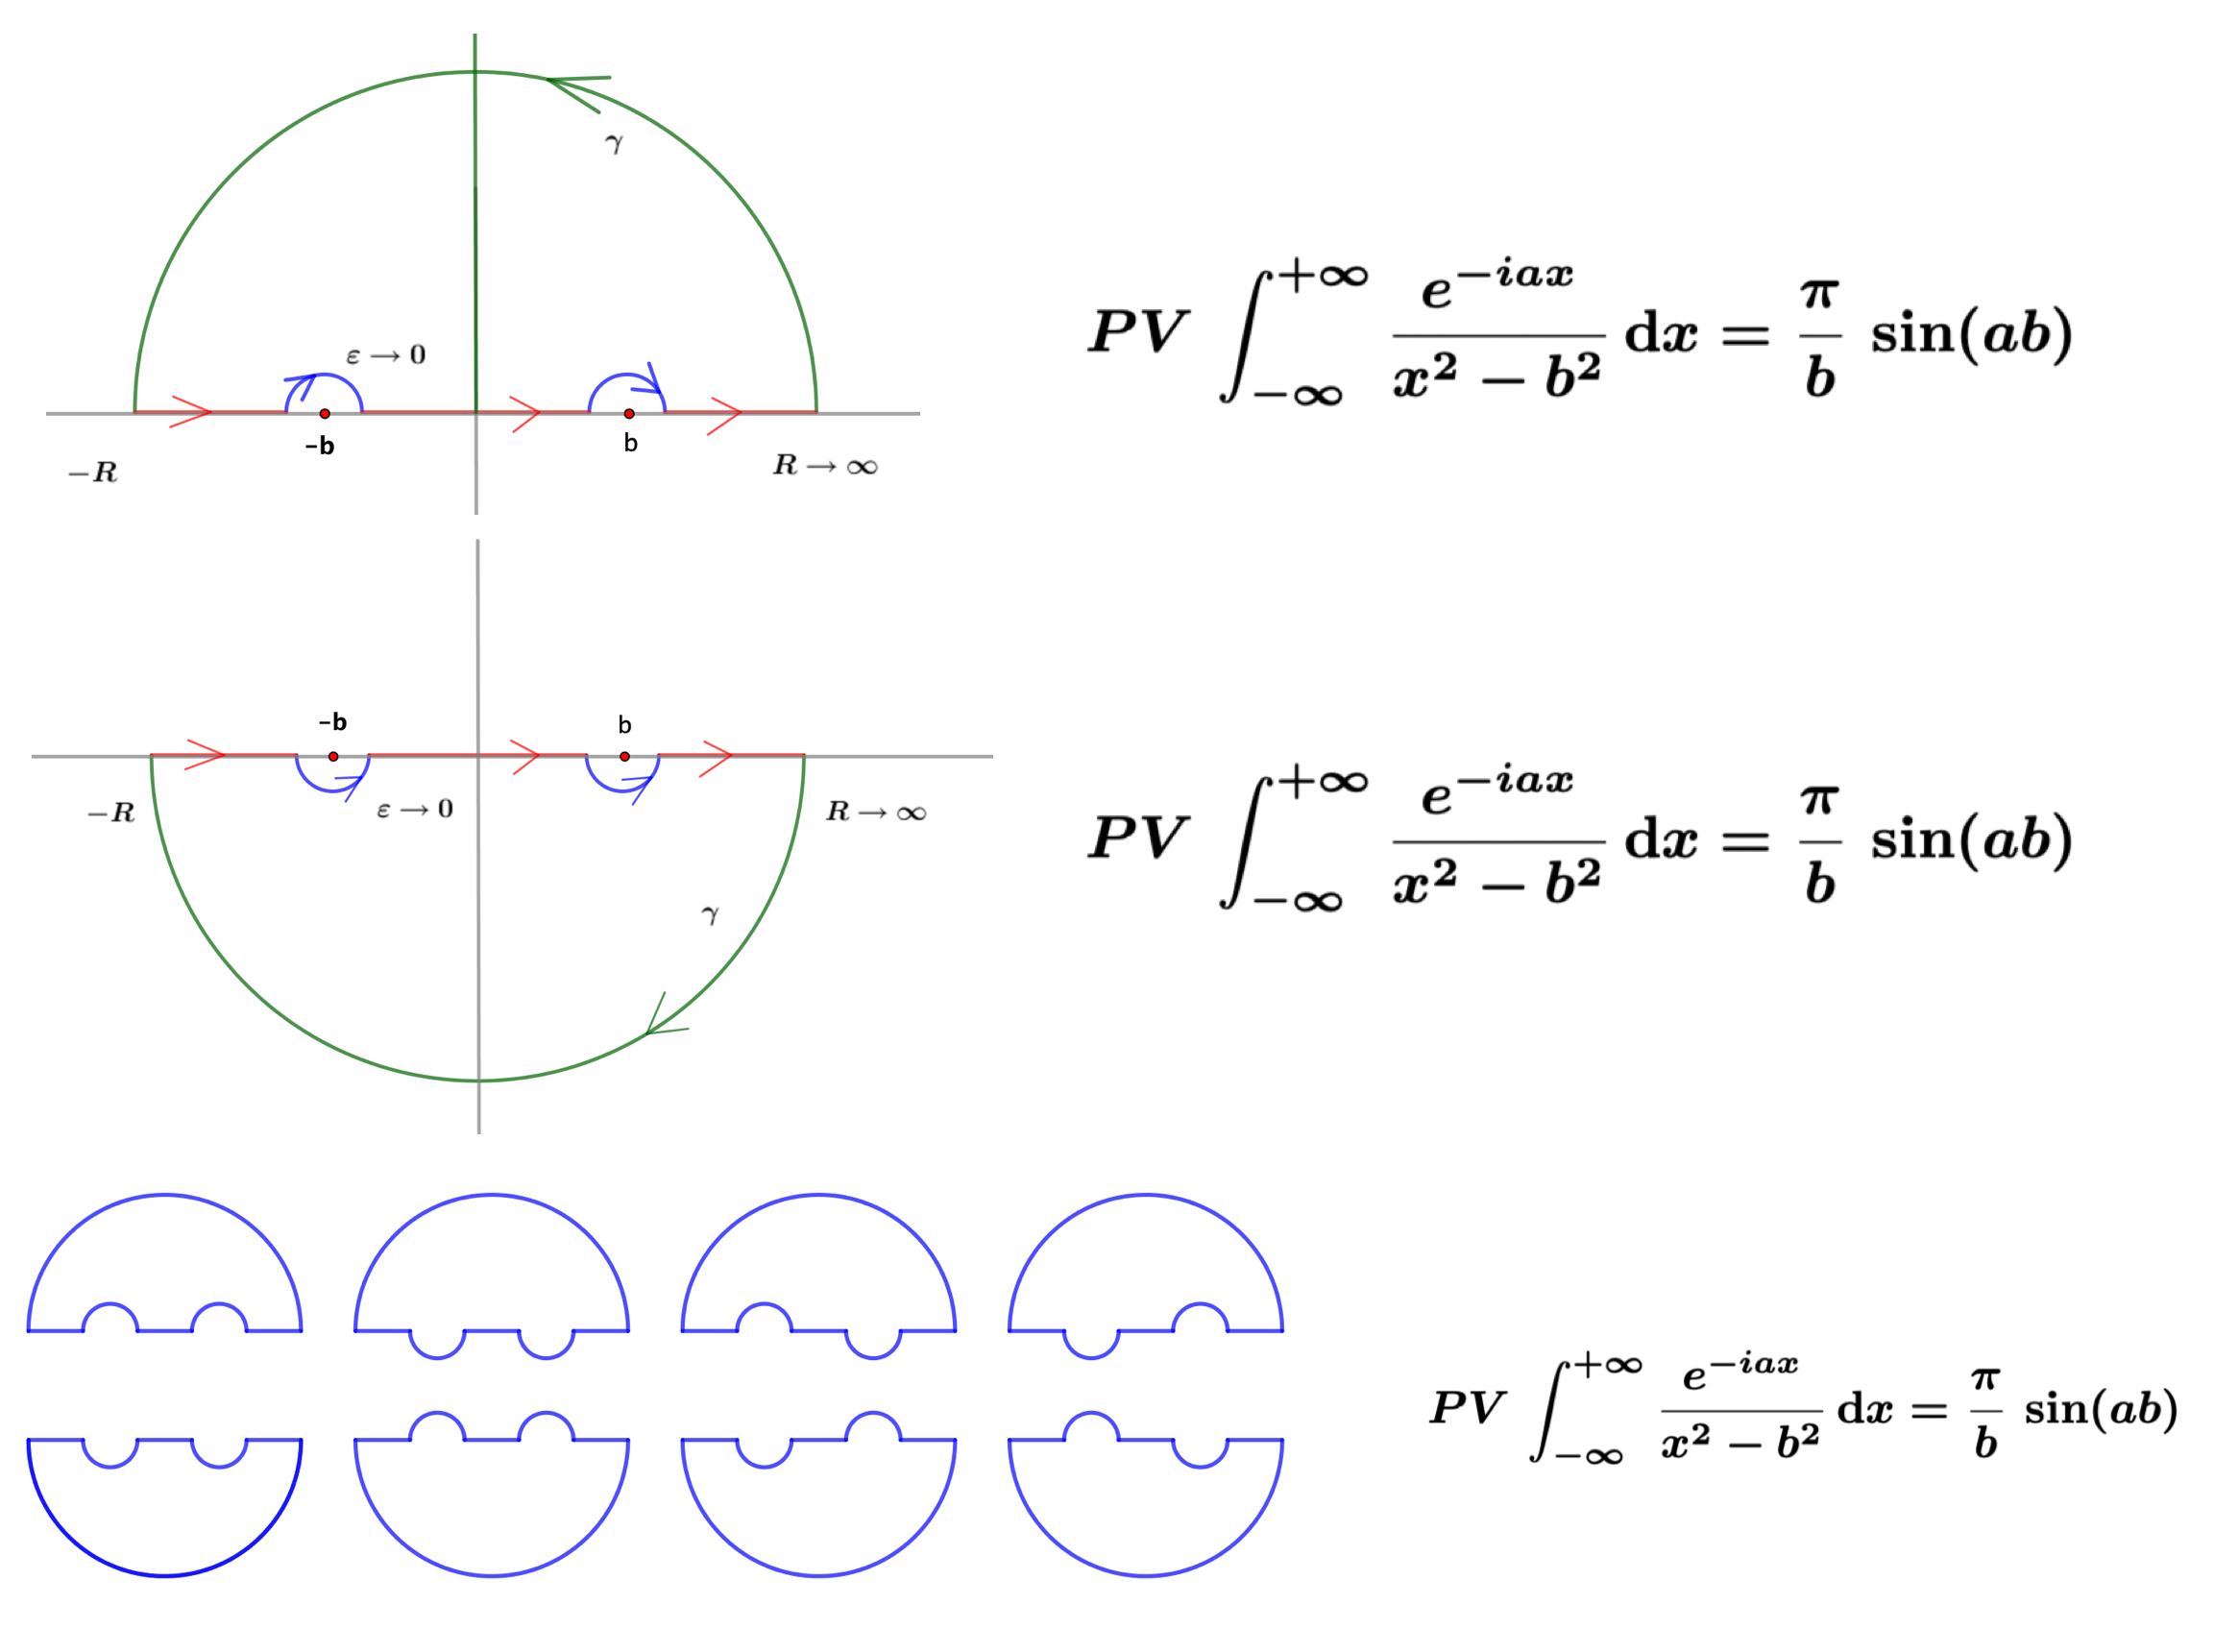
\includegraphics[width=.85\textwidth]{imagenes/img43-04.png}
 \end{figure}

\vspace{5mm}
\section{Regularización de Feynman o $\boldsymbol{\ +i\varepsilon\ \textit{prescription}}$} 

Ahora no deformaremos el entorno a la hora de integrar, para regularizar la presencia de los polos reales en $\pm b$ sustituiremos la integral de partida, $\int_{-\infty}^{+\infty}  \dd x \, {e^{-iax}}/({x^2-b^2}) \, , \ $  por otra diferente.

Nos inventamos una nueva función que tendrá los ejes fuera del eje real.

 \begin{figure}[H]
	\centering
	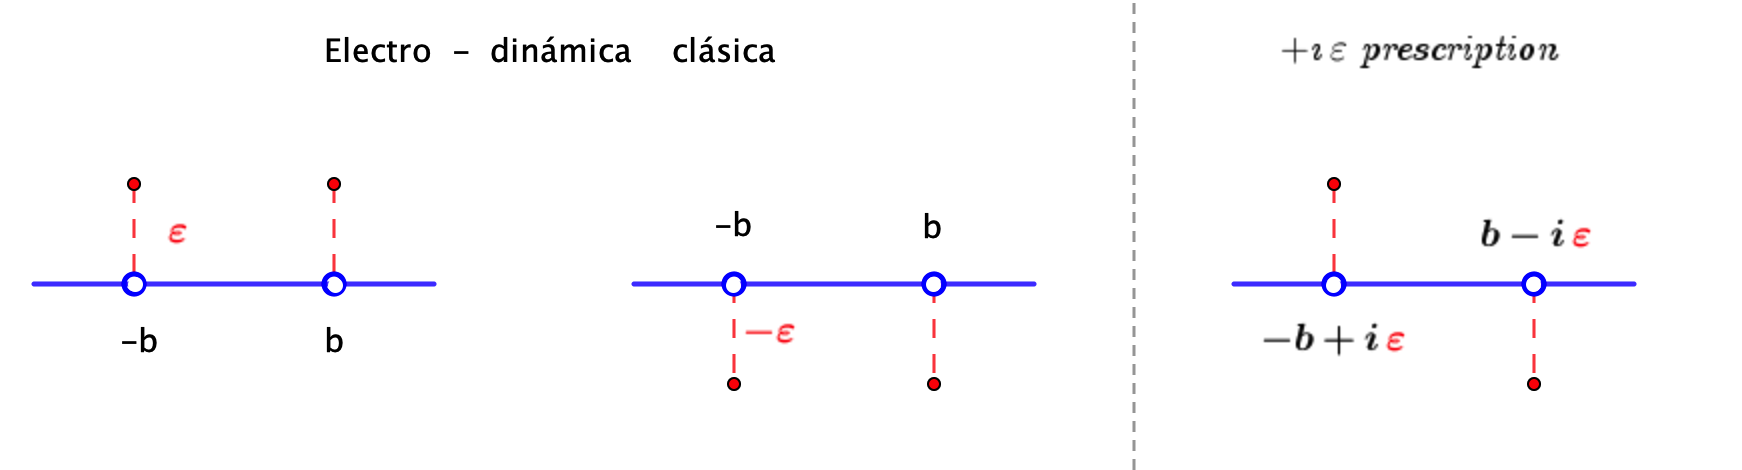
\includegraphics[width=.95\textwidth]{imagenes/img43-05.png}
 \end{figure}

--- Si elegimos que los dos polos estén por encima del eje real, o por abajo, estamos adoptando la opción de la \emph{electrodinámica clásica}.

--- La opción de \emph{Feynman} consiste en tomar un polo por arriba y otro por abajo.



El denominador de la función del integrando será, ahora,

$\, z-(-b+i\varepsilon)\, ) \cdot (\, z-(b-i\varepsilon)\, ) = z^2-z(b-i\varepsilon)-z(-b+i\varepsilon)+(-b+i\varepsilon)(b-i\varepsilon)=z^2-z(\cancel{b}-\bcancel{i\varepsilon}-\cancel{b}+\bcancel{i\varepsilon})-(b-i\varepsilon)^2= z^2-(b^2-2bi\varepsilon -\cancelto{0}{\varepsilon^2})=z^2-b^2+2bi\varepsilon  \qquad \qquad \varepsilon \text{ infinitesimal : } \quad \varepsilon<<1 \ \to \ \varepsilon^2 \approx 0$

Ahora consideramos la integral: $\quad \displaystyle \oint \dd z \, \dfrac{e^{-iaz}}{z^2-b^2+2i\varepsilon}$

Calculemos los residuos:

$\displaystyle \lim_{z\to -b+i\varepsilon} (\, z-(-b+i\varepsilon)\, ) \,  \dfrac{e^{-iaz}}{z^2-b^2+i2b\varepsilon} = \textcolor{gris}{ (\, \dfrac 0 0\, \text{ L'Hôpital }\, ) } = e^{ia(-b+i\varepsilon)}\, \lim_{z\to -b+i\varepsilon}  \dfrac{1}{2z} =  e^{ia(-b+i\varepsilon)}\, \dfrac{1}{2(-b+i\varepsilon)}$

Tomando límites cuando $\varepsilon$ tiende a cero: $\displaystyle \ \boldsymbol{ \Res(f(z),-b)}= \lim_{\varepsilon \to 0}  e^{ia(-b+i\varepsilon)}\, \dfrac{1}{2(-b+i\varepsilon)} = \boldsymbol{ \dfrac{e^{iab}}{-2b}}\, . \ $ Análogamente, $\ \boldsymbol{ \Res(f(z),b)=  \dfrac{e^{-iab}}{2b}} $


\begin{small} \textcolor{gris}{
	$\displaystyle \Res(f(z),b)=\lim_{\varepsilon\to 0} \lim_{z\to b-i\varepsilon} \cancel{(z-(b-i\varepsilon))} \dfrac{e^{-ia(b-i\varepsilon))}} {\cancel{(z-(b-i\varepsilon)}(z-(b+i\varepsilon)}=\  (\, 0/0\, \text{L'H}\, ) \ = \lim_{\varepsilon\to 0} \dfrac { e^{-iab-a\varepsilon} }{2(b-i\varepsilon)}= \dfrac{e^{-iab}}{2b}$  } \end{small}

$\triangleright \quad \boldsymbol{ \boxed{\ a<0\ }} \quad $ Consideremos ahora, para la integral, un circuito que cierra el contorno por arriba (sin deformarlo)

$\displaystyle \textcolor{red}{\int_{-\infty}^{\infty} \, \boldsymbol I} \, + \, \cancelto{0}{\int_{R\to \infty}}\ = \ \int_\gamma \ = \ 2\pi \sum (\text{residuos internos}) \ = \ 2\pi \, \dfrac{e^{iab}}{-2b}$

$$\boldsymbol{ I \ = \ - \dfrac{\pi\, i}{2} \, e^{iab} } \qquad \quad \boldsymbol{a<0}$$

\begin{figure}[H]
	\centering
	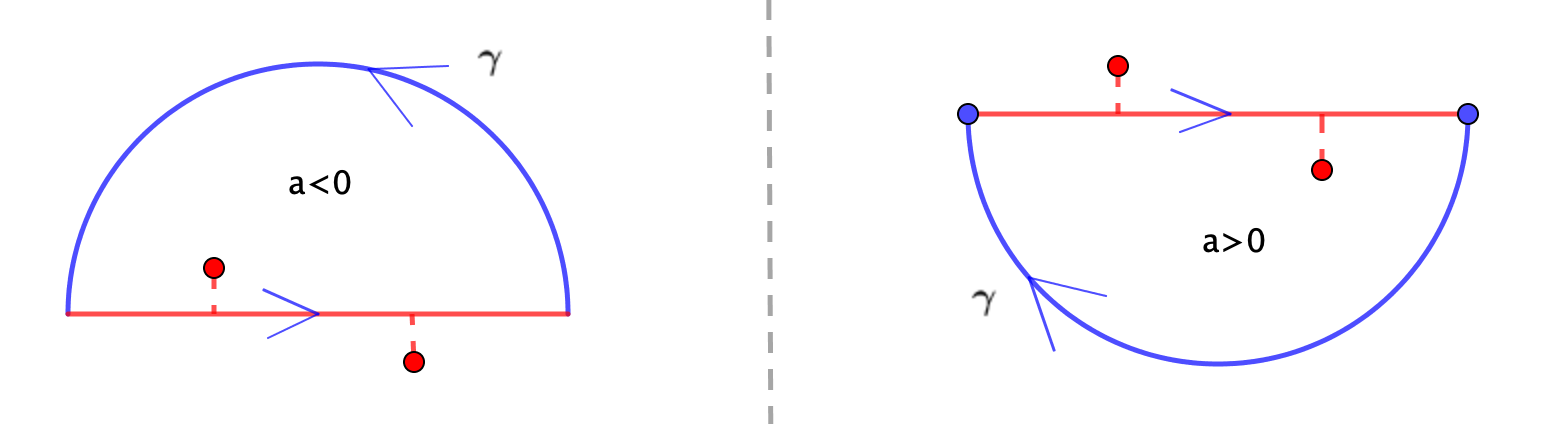
\includegraphics[width=.95\textwidth]{imagenes/img43-06.png}
 \end{figure}
 
 $\triangleright \quad \boldsymbol{ \boxed{\ a>0\ }} \quad $ Consideremos ahora, para la integral, un circuito que cierra el contorno por abajo (sin deformarlo)
 
 $$\boldsymbol{ I \ = \ - \dfrac{\pi\, i}{2} \, e^{-iab} } \qquad \quad \boldsymbol{a>0}$$
 
 Una forma compacta de escribir ambos resultados en una línea en usando $\ -|a| = \begin{cases} \ -a & a\ge 0 \\ \ \ a  & a< 0 \end{cases}$,
 
 $$\displaystyle \boldsymbol{
 \int_{-\infty}^{+\infty}  \dd z \, \dfrac {e^{-iaz}}{z^2-b^2+i2b\varepsilon} \ = \  - \dfrac{\pi\, i}{2} \, e^{-i\, b\,|a|} 
 }$$
 
 Aún más, podemos sustituir $\ 2v\varepsilon \ $ por $\ \varepsilon' \ $, es como si en vez de desplazar una distancia $\varepsilon$ los polos los hiciésemos una distancia $\ \varepsilon/2b\ $; incluso podemos llamar $\varepsilon$ al $\varepsilon'$ que hemos cambiado y as-i es como aparece en los textos la ...
 
 \vspace{5mm}
 \begin{large}
 \begin{myblock}{Prescripción de Feynman }
 \begin{equation}
 \label{T43PF}
 \boldsymbol{
 \int_{-\infty}^{+\infty}  \dd z \ \dfrac {e^{-iaz}}{z^2-b^2+i\varepsilon} \ = \  - \dfrac{\pi\, i}{2} \, e^{-i\, b\,|a|} 
 }	
 \end{equation}	
 \end{myblock}
 \end{large}

\vspace{10mm}
\color{gris}

Tenemos $\quad \displaystyle  \int_{-\infty}^{+\infty}  \dd z \ \dfrac {e^{-iaz}}{z^2-b^2+i\varepsilon} \ = \  - \dfrac{\pi\, i}{2} \, e^{-i\, b\,|a|}  \qquad \qquad  \text{Cambio de variable:}\quad \varepsilon'=2b\varepsilon$

$b$ es una constante fija por lo que $\ \varepsilon\to 0 \ \Rightarrow \  \varepsilon' \to 0$

$I= \int_{-\infty}^{+\infty}  \dd z \, \dfrac {e^{-iaz}}{z^2-b^2+i\varepsilon'} \ = \  - \pi \, i \,  \dfrac { e^{ -i \left( b-i\dfrac{\varepsilon'}{2b} \right)\, |a| } } {b-i \dfrac{\varepsilon'}{2b}} \, 
\begin{matrix} \\ \longrightarrow \\ \varepsilon'\to 0 \end{matrix}
\, -\dfrac{\pi\, i}{b}\ e^{-i\, b\, |a|}$

Volviendo a llamar $\varepsilon$ a $\varepsilon'$, tendremos la ``prescription $+i\varepsilon$''


\color{black} 
